%!TEX root=./LIVRO.tex
\pagebreak

\mbox{}

\begin{figure}
\vspace*{-3cm}
\hspace*{-3.7cm}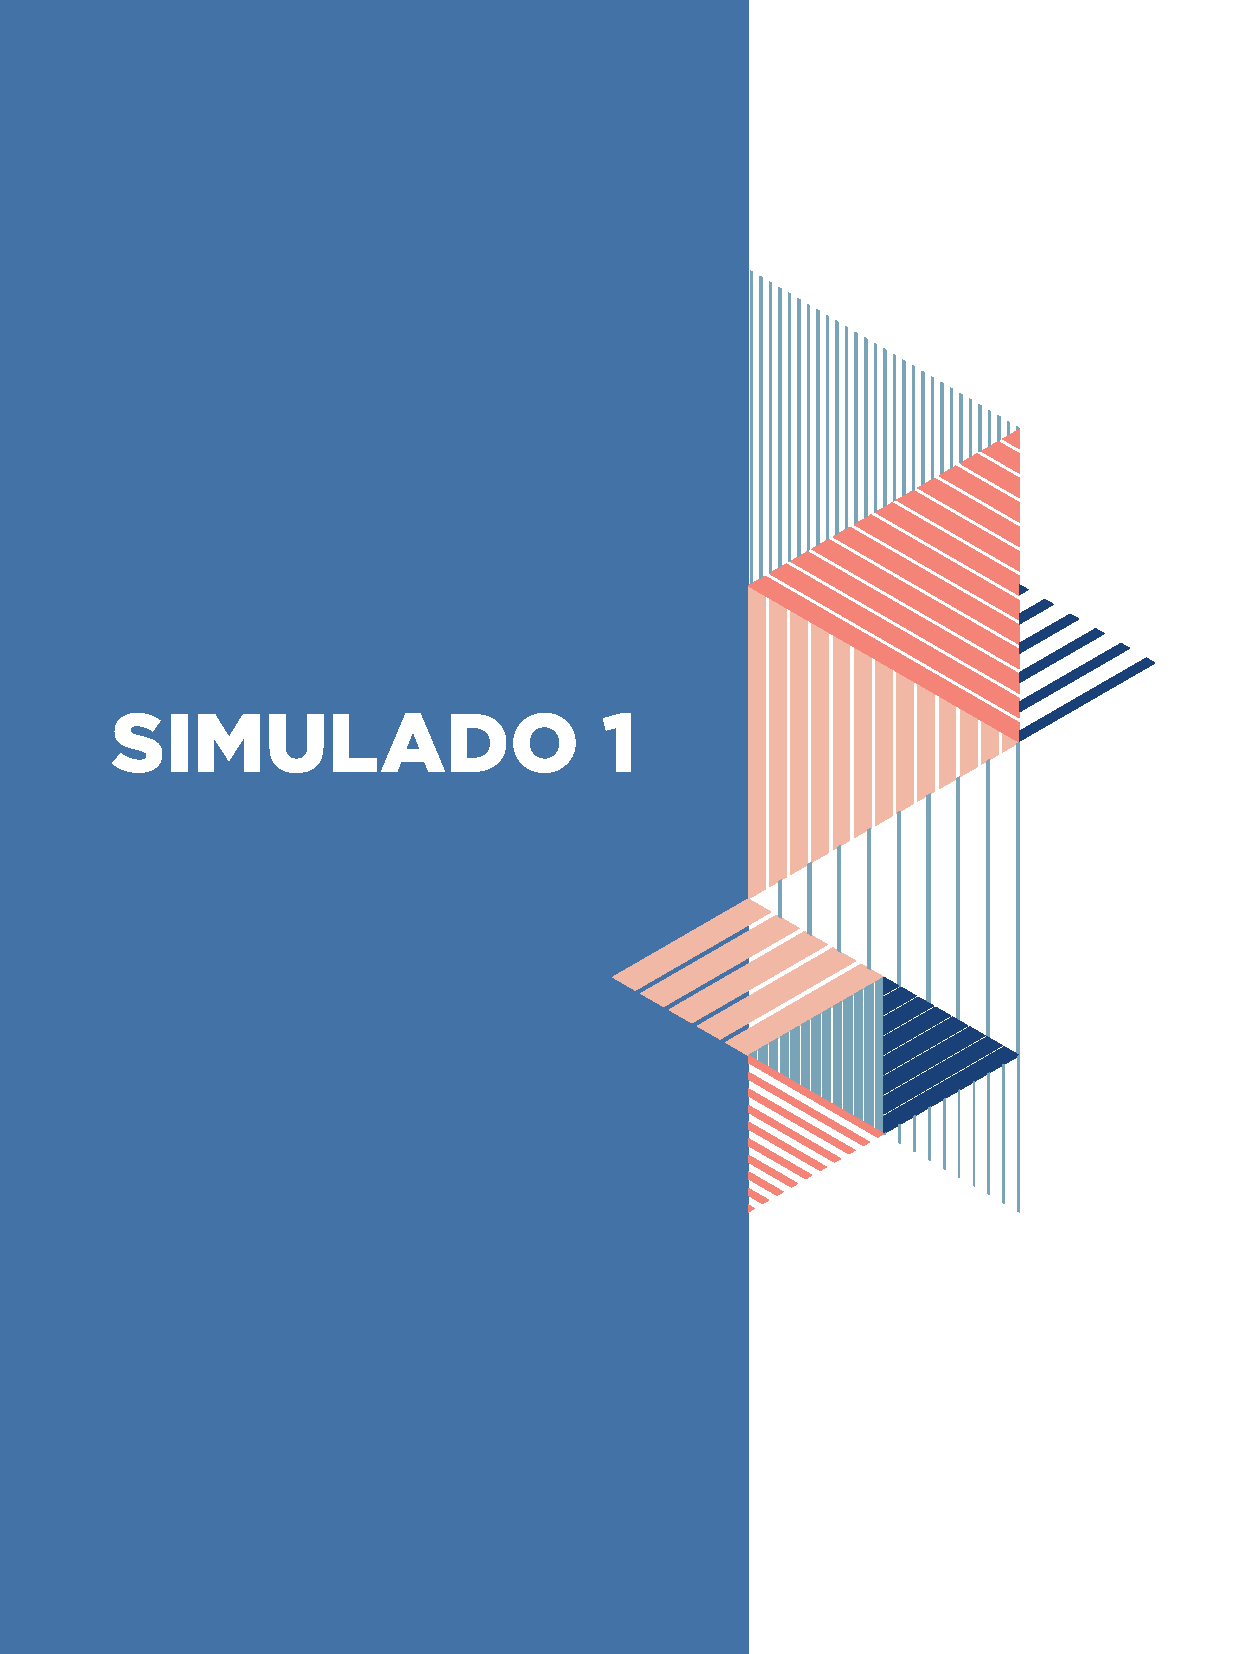
\includegraphics[scale=1]{../watermarks/1simulado9ano.pdf}
\end{figure}


\pagebreak

\section*{Simulado 1}

\num{1} Uma escola organizou uma corrida com obstáculos. Respectivamente,
Júlio, Tiago, Isabel e Fábio obtiveram os tempos:
13,02  - 14,89  - 14,62  - 14,7. Marque a opção em que os
tempos são ordenados numa crescente.

\begin{escolha}
\item Tiago - Fábio- Júlio - Isabel
\item Fábio - Isabel - Júlio - Tiago
\item Júlio - Isabel - Fábio - Tiago
\item Júlio - Isabel - Tiago - Fábio
\end{escolha}

%\section{BNCC: EF07MA10 }
% -- Comparar e ordenar números racionais em diferentes
% contextos e associá-los a pontos da reta numérica.
% SAEB: Comparar ou ordenar números reais, com ou sem suporte da reta
% numérica, ou aproximar número reais para múltiplos de potência de 10
% mais próxima.

% A - Incorreta, pois Fábio fez em um tempo menor que Tiago e veio depois
% na listagem.
% B - Incorreta, pois Isabel fez em um tempo menor que Fábio e veio depois
% na listagem.
% C - Correta, pois os números que possuem as partes inteiras iguais foram
% analisados pelas casas decimais.
% D - Incorreta, pois, apesar de Júlio e Isabel estarem nas posições
% corretas, o Fábio fez um tempo menor que Tiago, logo, ele não seria o
% último.

\num{2} A solução para a expressão
$17 + ( - 2) \times { 5 - 9 + 2 \times \lbrack 36 \div 4 - ( 7 \times 3 ) \rbrack }$
é:

\begin{escolha}
\item -420
\item 420
\item - 79
\item 73
\end{escolha}

%\section{BNCC: EF07MA04 }
% -- Resolver e elaborar problemas que envolvam operações
% com números inteiros.
% SAEB: Calcular o resultado de adições, subtrações, multiplicações ou
% divisões envolvendo números reais.

% A - Incorreta, pois resolveu
% 17 + ( - 2) \times \left( - 28 \right) = 15 \times ( - 28) = - 420.
% B - Incorreta, pois resolveu
% 17 + ( - 2) \times \left( - 28 \right) = - 15 \times ( - 28) = 420. 
% C - Incorreta, errou no jogo de sinal e resolveu pois resolveu que
% ( - 2) \times \left( - 28 \right) = \  - 96.
% D - Correta, pois
% 17 + ( - 2) \times \left\{ - 4 + 2 \times \left\lbrack 9 - \left( 21 \right) \right\rbrack \right\} = 17 + ( - 2) \times \left\{ - 4 - 24 \right\} = 17 + ( - 2) \times \left( - 28 \right) = 73.

\num{3} O tio de Juliana é 20 anos mais velho que ela. Considerando que
Leandro foi pai de Juliana com 23 anos e hoje está com 39 anos, qual é a
idade do tio de Juliana?

\begin{escolha}
\item 36
\item 22
\item 25
\item 35
\end{escolha}

%\section{BNCC: EF07MA18 }
% -- Resolver e elaborar problemas que possam ser
% representados por equações polinomiais de 1º grau, redutíveis à forma ax
% + b = c, fazendo uso das propriedades da igualdade.
% SAEB: Resolver uma equação polinomial de 1º grau.

% A - Correta, pois J + 20 = \ \text{Tio}; J = 39 - 23 = 16; 16 + 20 = 36.
% B - Incorreta, pois, se Juliana tivesse 22 anos, seu tio teria 42 anos,
% o que não condiz com o enunciado.
% C - Incorreta, pois, se Juliana tivesse 25 anos, seu tio teria 45 anos,
% o que não condiz com o enunciado.
% D - Incorreta, pois, se Juliana tivesse 35 anos, seu tio teria 55 anos,
% o que não condiz com o enunciado.

\num{4} Marcela estava acompanhando o preço de um produto desde janeiro,
quando ele custava R\$2.100,00. Em março, ela observou que houve um
aumento de 10\% do valor. Em maio, foi dado um desconto de 12\%. Marcela
comprou o produto em junho, quando percebeu um novo aumento de 5\%.
Comparado com o preço de janeiro, Marcela comprou o produto com

\begin{escolha}
\item aumento de, aproximadamente, 16\%.
\item desconto de, aproximadamente, 16\%.
\item aumento de, aproximadamente, 1,6\%.
\item desconto de, aproximadamente, 1,6\%.
\end{escolha}


%\section{BNCC: EF07MA02 }
% -- Resolver e elaborar problemas que envolvam
% porcentagens, como os que lidam com acréscimos e decréscimos simples,
% utilizando estratégias pessoais, cálculo mental e calculadora, no
% contexto de educação financeira, entre outros.
% SAEB: Resolver problemas que envolvam porcentagens, incluindo os que
% lidam com acréscimos e decréscimos simples, aplicação de percentuais
% sucessivos e determinação de taxas percentuais.

% A - Incorreta, pois considerou que 0,0164\cong 16\%
% B - Incorreta, pois além de considerar 0,0164\cong 16\%,
% interpretou como desconto.
% C - Correta, pois, fazendo os cálculos com os fatores de multiplicação,
% temos 1,1 \times 0,88 \times 1,05 = 1,0164 - 1 = 0,0164\cong 1,6\%.
% D - Incorreta, pois fez as contas de forma correta, mas interpretou como
% desconto ao invés de aumento.

\num{5} Rogério, Fernanda, Otávio foram em um rodízio de pizza e comeram o
equivalente ao que está pintado na figura. Qual fração representa essa
quantidade?

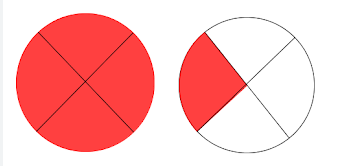
\includegraphics[width=3.625in,height=1.72917in]{./imgSAEB_7_MAT/media/image95.png}

\begin{escolha}
\item $\frac{5}{6}$
\item $3\frac{1}{4}$
\item $1\frac{1}{4}$
\item $1\frac{4}{4}$
\end{escolha}

%\section{BNCC: EF07MA09 }
% -- Utilizar, na resolução de problemas, a associação
% entre razão e fração, como a fração 2/3 para expressar a razão de duas
% partes de uma grandeza para três partes da mesma ou três partes de outra
% grandeza.
% SAEB: Representar frações menores ou maiores que a unidade por meio de
% representações pictóricas ou associar frações a representações
% pictóricas.

% A - Incorreta, pois a quantidade de fatias pintadas está correta, porém,
% o denominador não condiz, uma vez, que é dividido em 4 partes.
% B - Incorreta, pois, embora a fração \frac{1}{4} apareça, a parte
% inteira tem somente um círculo todo pintado.
% C - Correta, pois apresenta 1 círculo todo pintado, que é a parte
% inteira e \frac{1}{4} de outro.
% D- Incorreta, pois a representação da parte inteira e da parte decimal,
% corresponde a 1 inteiro, logo 2 inteiros, e na imagem somente um círculo
% está todo pintado.

\num{6} Na aula de matemática de Sofia, a professora escreveu a sequência
abaixo no quadro e pediu para os alunos escreverem a lei de formação de
acordo com a posição dos termos.

2,\ 6,\ 12,\ 20,\ldots

Sofia conseguiu encontrar a lei de formação correta, sendo ela:

\begin{escolha}
\item $a_{n} = 2n + 2$
\item $a_{n} = n² + n$
\item $a_{n} = 4n$
\item $a_{n} = n(n - 1)$
\end{escolha}

%%\section{BNCC: EF07MA15 }
% -- Utilizar a simbologia algébrica para expressar
% regularidades encontradas em sequências numéricas.
% SAEB: Identificar uma representação algébrica para o padrão ou a
% regularidade de uma sequência de números racionais ou representar
% algebricamente o padrão ou a regularidade de uma sequência de números
% racionais.

% A - Incorreta, pois o primeiro termo seria
% a_{1} = 2 \times 1 + 2 = 2 + 2 = 4, o que não confere.
% B - Correta., pois temos, a_{1} = 1^{2} + 1 = 1 + 1 = 2,
% a_{2} = 2^{2} + 2 = 4 + 2 = 6, a_{3} = 3^{2} + 3 = 9 + 3 = 12 e
% a_{4} = 4² + 4 = 16 + 4 = 20.
% C - Incorreta, pois o primeiro termo seria a_{1} = 4 \times 1 = 4, o
% que não confere.
% D - Incorreta, pois o primeiro termo seria
% a_{1} = 1\left( 1 - 1 \right) = 1 \times 0 = 0, o que não confere.

\num{7} Em uma brincadeira, ganha aquele que encontrar o sete de copas em um
baralho. Lucas começou jogando e tirou duas cartas, nenhuma delas sendo
o sete de copas. Qual é a probabilidade de o próximo jogador ganhar?

\begin{escolha}
\item $\frac{3}{52}$
\item $\frac{1}{2650}$
\item $\frac{1}{52}$
\item $\frac{1}{2600}$
\end{escolha}

%%\section{BNCC: EF07MA34 }

% -- Planejar e realizar experimentos aleatórios ou
% simulações que envolvem cálculo de probabilidades ou estimativas por
% meio de frequência de ocorrências.
% SAEB: Resolver problemas que envolvam a probabilidade de ocorrência de
% um resultado em eventos aleatórios equiprováveis independentes ou
% dependentes.

% A - Incorreta, pois calculou a probabilidade com 3 cartas,
% desconsiderando os eventos e a independência entre eles.
% B - Incorreta, pois não considerou que foram retiradas 2 cartas de uma
% vez.
% C - Incorreta, pois calculou apenas a probabilidade do primeiro evento
% acontecer.
% D - Correta, pois são eventos dependentes. A primeira jogada influencia
% na segunda jogada: P\left( A \right) = \frac{1}{52};\ P\left( A \right) = \frac{1}{50}; P\left( A \right) \times P\left( A \right) = \frac{1}{52} \times \frac{1}{50} = \frac{1}{2600}.

\num{8} Um carro faz uma viagem em 5 horas andando a 120km/h. Porém, o
trajeto foi modificado e o limite de velocidade passou a ser de 100km/h.
Quanto tempo esse carro gastará no trajeto com essa nova velocidade?

\begin{escolha}
\item 5 horas
\item 6 horas
\item 4 horas e 9 minutos
\item 4 horas e 10 minutos
\end{escolha}


%\section{BNCC: EF07MA17 }
% -- Resolver e elaborar problemas que envolvam variação de
% proporcionalidade direta e de proporcionalidade inversa entre duas
% grandezas, utilizando sentença algébrica para expressar a relação entre
% elas.
% SAEB: Resolver problemas que envolvam variação de proporcionalidade
% direta~ou inversa entre duas ou mais grandezas.

% A - Incorreta, pois considerou que, mesmo mudando a velocidade, o tempo
% permaneceria o mesmo.
% B - Correta, pois velocidade e tempo são grandezas inversamente
% proporcionais, logo, o produto entre elas é constante. Assim,
% 5 \times 120 = 100x \rightarrow 100x = 600 \rightarrow x = \frac{600}{100} = 6\ h\text{oras}.
% C - Incorreta, pois considerou as grandezas como diretamente
% proporcionais e ainda arredondou 4,16 horas para 4 horas e 9 minutos.
% D - Incorreta, pois considerou as grandezas como diretamente
% proporcionais.

\num{9} Em uma pesquisa qualitativa nominal, foram apresentados dados da cor
dos olhos da amostra escolhida. O gráfico era todo colorido dentro de um
círculo dividido em fatias. Qual tipo de gráfico é esse?

\begin{escolha}
\item
  Histograma
\item
  Gráfico de barras
\item
  Gráfico de colunas
\item
  Gráfico de linhas
\end{escolha}

%%\section{BNCC: EF07MA37}
%  -- Interpretar e analisar dados apresentados em gráfico
% de setores divulgados pela mídia e compreender quando é possível ou
% conveniente sua utilização.
% SAEB: Representar ou associar os dados de uma pesquisa estatística ou de
% um levantamento em listas, tabelas (simples ou de dupla entrada) ou
% gráficos (barras simples ou agrupadas, colunas simples ou agrupadas,
% pictóricos, de linhas, de setores, ou em histograma).

% A - Incorreta, pois o histograma é feito por linhas e barras.
% B - Incorreta, pois o gráfico de barras é formado por barras
% retangulares e com base maior na horizontal.
% C - Correta, pois esse tipo de gráico apresenta setores de uma figura
% geométrica, geralmente, um círculo.
% D - Incorreta, pois o gráfico de linhas é representado por pontos unidos
% por linhas.

\num{10} No plano cartesiano, considere o triângulo ABC com vértices A(2, 4),
B(5, 6) e C(7, 2). A figura obtida após aplicar uma transformação de
reflexão em relação ao eixo x nesse triângulo será:

\begin{escolha}
\item Triângulo A'B'C' com vértices A'(-2, 4), B'(5, -6) e C'(7, -2)
\item Triângulo A'B'C' com vértices A'(-2, -4), B'(5, -6) e C'(7, -2)
\item Triângulo A'B'C' com vértices A'(-2, -4), B'(5, 6) e C'(7, 2)
\item Triângulo A'B'C' com vértices A'(2, -4), B'(-5, -6) e C'(-7, -2)
\end{escolha}

%\section{BNCC: EF07MA20 }
% -- Reconhecer e representar, no plano cartesiano, o
% simétrico de figuras em relação aos eixos e à origem.
% SAEB: Identificar, no plano cartesiano, figuras obtidas por uma ou mais
% transformações geométricas (reflexão, translação, rotação).

% A - Incorreta, pois os valores dos vértices não condizem com o processo
% de reflexão.
% B - Correta, pois, ao realizar uma reflexão em relação ao eixo x, os
% pontos mantêm a mesma coordenada x, mas têm sua coordenada y negativa.
% No triângulo ABC original, o ponto A(2, 4) terá a mesma coordenada x,
% mas sua coordenada y será negativa, resultando em A'(-2, -4). Da mesma
% forma, os pontos B(5, 6) e C(7, 2) terão suas coordenadas y negativas
% após a reflexão, resultando em B'(5, -6) e C'(7, -2), respectivamente.
% C - Incorreta, pois os valores dos vértices não condizem com o processo
% de reflexão.
% D - Incorreta, pois os valores dos vértices não condizem com o processo
% de reflexão.

\num{11} No triângulo ABC, o ângulo A é um ângulo reto e o lado AC mede 5 cm.
Se o ângulo B mede 45 graus, qual é o comprimento do lado BC?

\begin{escolha}
\item
  5 cm
\item
  5 $\sqrt{2}$ cm
\item
  5 $\sqrt{3}$cm
\item
  10 cm
\end{escolha}


%\section{BNCC: EF07MA24 }
% -- Construir triângulos, usando régua e compasso,
% reconhecer a condição de existência do triângulo quanto à medida dos
% lados e verificar que a soma das medidas dos ângulos internos de um
% triângulo é 180°.
% SAEB: Identificar propriedades e relações existentes entre os elementos
% de um triângulo.

% A - Correta, pois pois o comprimento do lado BC é igual ao comprimento
% do lado AC em um triângulo retângulo com ângulos de 45 graus.
% B - Incorreta, pois essa resposta seria correta se o triângulo fosse um
% triângulo isósceles retângulo de 45-45-90 graus, mas no problema não foi
% mencionado que os ângulos são iguais.
% C - Incorreta, pois essa resposta seria correta se o triângulo fosse um
% triângulo equilátero de 60 graus, mas no problema não foi mencionado que
% os ângulos são iguais.
% D - Incorreta, pois essa resposta é o dobro do comprimento do lado AC, o
% que não é possível em um triângulo retângulo com ângulos de 45 graus.

\num{12} Observe a imagem abaixo onde ocorreu o deslocamento do retângulo
ABCD.

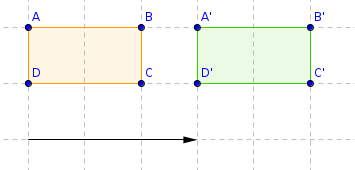
\includegraphics{./imgSAEB_7_MAT/media/image98.png}

Considerando que cada quadrado da malha tem 1 cm de lado, o deslocamento
do retângulo foi de:

\begin{escolha}
\item
  1 cm para a direita
\item
  3 cm para a direita
\item
  1 cm para a esquerda
\item
  3 cm para a esquerda
\end{escolha}

% SAEB: Descrever ou esboçar deslocamento de pessoas e/ou de objetos em
% representações bidimensionais (mapas, croquis etc.), plantas de
% ambientes ou vistas, de acordo com condições dadas.

% A - Incorreta, pois considerou a distância das duas imagens como o total
% do deslocamento.
% B - Correta, pois, pegando o vértice A como referência, podemos observar
% que ele foi deslocado em três espaços para a direita, gerando o vértice
% A'. Como cada linha da malha é 1 cm, o total do deslocamento foi de 3 cm
% para a direita.
% C - Incorreta, pois, além de considerar a distância das duas imagens
% como o total do deslocamento, confundiu a direção.
% D - Incorreta, pois fez o deslocamento correto, mas confundiu a direção.

\num{13} Frederico e Paulo estão pesquisando o preço de motos. A alternativa
que eles encontraram foi comparar a venda de quatro marcas diferentes
durante três meses. O critério de escolha será a maior média. Qual marca
eles compraram?

\begin{longtable}[]{@{}llll@{}}
\toprule
aulo: cria & r uma tabela com as infor & mações abaixo: &\tabularnewline
\midrule
\endhead
Marcas~ & Primeiro mês de vendas & Segundo mês de vendas & Terceiro mês
de vendas\tabularnewline
Yamaha & 12 & 8 & 13\tabularnewline
Suzuki & 7 & 4 & 10\tabularnewline
BMW & 2 & 6 & 14\tabularnewline
Honda & 8 & 3 & 7\tabularnewline
\bottomrule
\end{longtable}

\begin{escolha}
\item Yamaha
\item Suzuki
\item BMW
\item Honda
\end{escolha}


%\section{BNCC: EF07MA35 }
% -- Compreender, em contextos significativos, o
% significado de média estatística como indicador da tendência de uma
% pesquisa, calcular seu valor e relacioná-lo, intuitivamente, com a
% amplitude do conjunto de dados.
% SAEB: Calcular os valores de medidas de tendência central de uma
% pesquisa estatística (média aritmética simples, moda ou mediana).

% A - Correta, pois,
% Mé\text{dia}\ \text{yama}ha = \ \frac{12 + 8 + 13}{3} = 11.
% B - Incorreta, pois,
% \ Mé\text{dia}\ \text{Suzuki}\  = \ \frac{7 + 4 + 10}{3} = 7.
% C - Incorreta, pois,
% Mé\text{dia}\ \text{BMW} = \ \frac{2 + 6 + 14}{3} = 7,3.
% D - Incorreta, pois,
% Mé\text{dia}\ \text{Honda} = \ \frac{8 + 3 + 7}{3} = 6.

\num{14} Um recipiente de formato cúbico tem aresta de tamanho 9m. A
capacidade desse recipiente é de:

\begin{escolha}
\item 729 litros
\item 7.290 litros
\item 72.900 litros
\item 729.000 litros
\end{escolha}

%\section{BNCC: EF07MA29 }
% -- Resolver e elaborar problemas que envolvam medidas de
% grandezas inseridos em contextos oriundos de situações cotidianas ou de
% outras áreas do conhecimento, reconhecendo que toda medida empírica é
% aproximada.
% SAEB: Resolver problemas que envolvam medidas de grandezas em que haja
% conversões entre unidades mais usuais.

% A - Incorreta, pois considerou que a relação m³ é direta ao litro.
% B - Incorreta, pois converteu m³ para litro multiplicando por 10.
% C - Incorreta, pois converteu m³ para litro multiplicando por 100.
% D - Correta, pois o volume do cubo cprresponde ao tamanho da aresta
% elevado à terceira potência. Logo, V = 9^{3} = 729m³ . Como
% 1m^{3} = \ 1000\ L \rightarrow \ 729\ m³\  = \ 729.000 litros.

\num{15} Considerando a expressão algébrica $(5c = d)$, o valor de c para
$d = 75$ é:

\begin{escolha}
\item (70)
\item (375)
\item (80)
\item (15)
\end{escolha}

%\section{BNCC: EF07MA13 }
% -- Compreender a ideia de variável, representada por
% letra ou símbolo, para expressar relação entre duas grandezas,
% diferenciando-a da ideia de incógnita.
% SAEB: Resolver problemas que envolvam cálculo do valor numérico de
% expressões algébricas.

% A - Incorreta, pois ao calcular 5c = 75, passou o 5 subtraindo ao
% invés de dividindo.
% B - Incorreta, pois substituiu o valor de d no lugar de c.
% C - Incorreta, pois ao calcular 5c = 75, passou o 5 somando ao invés
% de dividindo.
% D - Correta, pois, para encontrar o valor de s, basta substituir o valor
% de t. Assim, 5c = d\  \rightarrow \ 5c = 75\  \rightarrow \ c = \frac{75}{5} = 15
\pagebreak

\mbox{}

\begin{figure}
\vspace*{-3cm}
\hspace*{-3.7cm}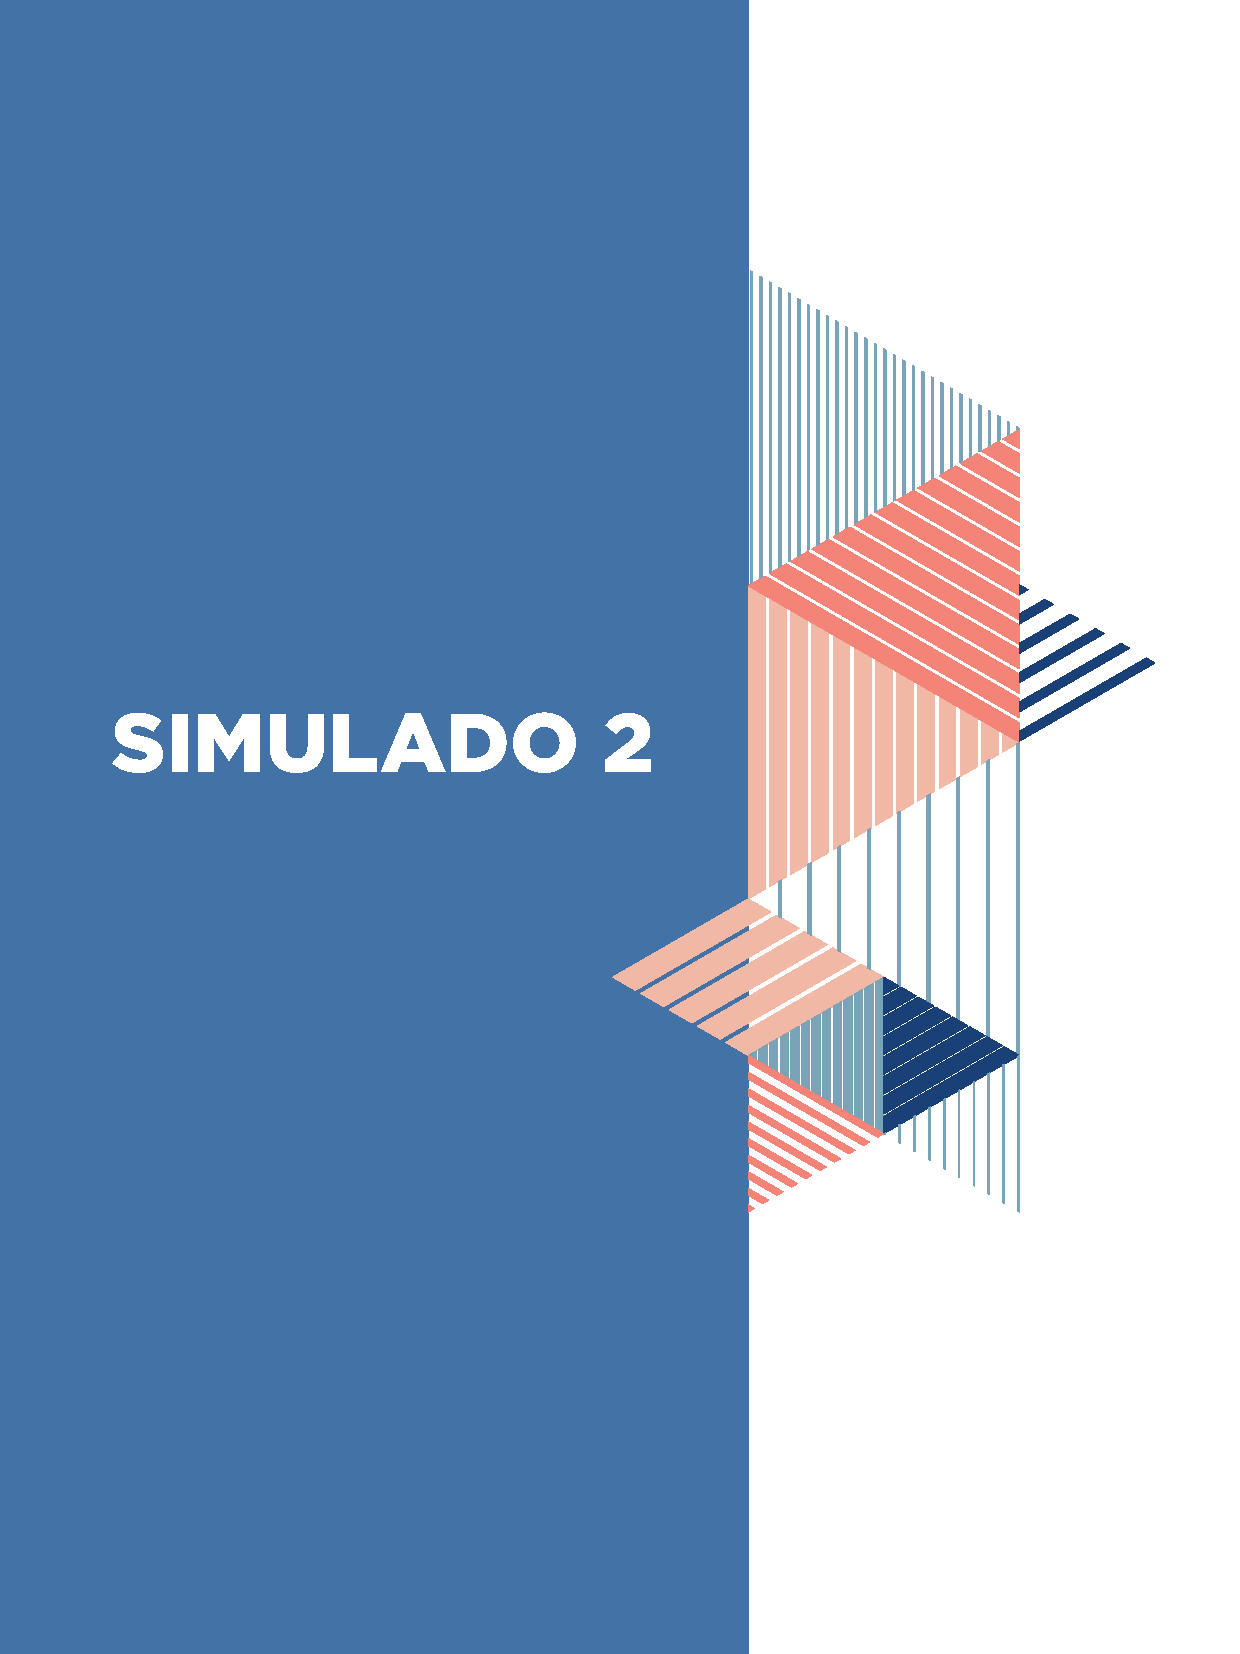
\includegraphics[scale=1]{../watermarks/2simulado9ano.pdf}
\end{figure}


\pagebreak

\section*{Simulado 2}

\num{1} Marcela vai fazer uma viagem para o exterior e precisa levar pelo
menos 300 combinações diferentes de looks para um ensaio fotográfico. Na
separação de roupas ela escolheu 5 blusas, 4 calças, 3 saias, 2 sapatos
e 3 blusas de frio. Usando essas opções Marcela vai conseguir a
quantidade de looks diferentes que precisa?

\begin{escolha}
\item Sim. Ainda vão sobrar 60 combinações de roupa.
\item Não. Ainda vão faltar 60 combinações de roupa.
\item Não. Ainda vão faltar 180 combinações de roupa..
\item Não, pois ela terá apenas 17 combinações possíveis de roupa.
\end{escolha}

%\section{BNCC: EF07MA04 }
% -- Resolver e elaborar problemas que envolvam operações
% com números inteiros.
% SAEB: Resolver problemas de contagem cuja resolução envolva a aplicação
% do princípio multiplicativo.

% A - Correta, pois, usando o princípio multiplicativo, as combinações
% distintas são 5 \times 4 \times 3 \times 2 \times 3 = 360. Como Marcela precisa de 300 combinações distintas, ainda vão sobrar 60
% opções de combinações.
% B - Incorreta, pois não percebeu que o número mínimo de combinações foi
% atingido.
% C - Incorreta, pois não considerou todas as peças de roupa.
% D - Incorreta, pois somou as opções de escolha ao invés de multiplicar.

\num{2} Mateus está vendendo seu telefone com 1 ano de uso. Fazendo uma
pesquisa, ele descobriu que o celular desvalorizou 20\% em relação ao
preço inicial. Sabendo que ele pagou R\$1.800,00, o preço atual é:

\begin{escolha}
\item R\$1.780,00
\item R\$1.440,00
\item R\$360,00
\item R\$1.400,00
\end{escolha}

%\section{BNCC: EF07MA02 }
% -- Resolver e elaborar problemas que envolvam
% porcentagens, como os que lidam com acréscimos e decréscimos simples,
% utilizando estratégias pessoais, cálculo mental e calculadora, no
% contexto de educação financeira, entre outros.
% SAEB: Resolver problemas que envolvam porcentagens, incluindo os que
% lidam com acréscimos e decréscimos simples, aplicação de percentuais
% sucessivos e determinação de taxas percentuais.

% A - Incorreta, pois considerou uma desvalorização de 20 reais.
% B - Correta, pois, como houve uma desvalorização de 20\%, vamos utilizar
% o fator multiplicativo 100\% - 20\% = 80\% = 0,8, assim 0,8 \times 1800 = 1440.
% C - Incorreta, pois considerou o valor da desvalorização e não o valor
% final.
% D - Incorreta, pois, ao fazer 1800 - 360, encontrou 1400 ao invés de
% 1440.

\num{3} Uma sequência equivalente a $a_{n} = n^2(n + 1)$ seria

\begin{escolha}
\item $a_{n} = n³(n + 1)$
\item $a_{n} = n(n² + 1)$
\item $a_{n} = n^{3} + n²$
\item $a_{n} = \ n³ + 1$
\end{escolha}

%\section{BNCC: EF07MA16 }
% -- Reconhecer se duas expressões algébricas obtidas para
% descrever a regularidade de uma mesma sequência numérica são ou não
% equivalentes.
%SAEB: Identificar representações algébricas equivalentes.

% A - Incorreta, pois considerou que, para duas sequências serem
% equivalentes, basta ter uma parte em comum.
% B - Incorreta, pois considerou que, ao trocar o n com n² de lugar, uma
% sequência semelhante seria gerada.
% C - Correta., pois, aplicando a propriedade distributiva, temos:
% n^{2}\left( n + 1 \right) = n^{3} + n^{2}.
% D - Incorreta, pois, ao fazer a distributiva, apenas multiplicou o n
% pelo n².

\num{4} Em um mapa, as instruções eram de que 10 cm no desenho correspondiam
a 10 km do real. Dessa forma, a escala utilizada é de:

\begin{escolha}
\item 1:10
\item 10:100000
\item 1:1000000
\item 1:100000
\end{escolha}

%\section{BNCC: EF07MA17 }
% -- Resolver e elaborar problemas que envolvam variação de
% proporcionalidade direta e de proporcionalidade inversa entre duas
% grandezas, utilizando sentença algébrica para expressar a relação entre
% elas.
% SAEB: Resolver problemas que envolvam variação de proporcionalidade
% direta ou inversa entre duas ou mais grandezas.

% A - Incorreta, pois considerou que basta igualar 1 cm no desenho ao
% mundo real.
% B - Incorreta, pois, ao simplificar \frac{10}{1000000}, foi colocado
% um 0 a mais no numerador.
% C - Incorreta, pois, ao simplificar \frac{10}{1000000}, foi colocado
% um 0 a mais no denominador.
% D - Correta, pois, como escala é a razão
% \frac{\text{desen}ho}{\text{real}} e ambos possuem a mesma unidade
% de medida, temos \frac{\text{desen}ho}{\text{real}} = \frac{10\text{cm}}{10\text{km}} = \frac{10}{1000000} = \frac{1}{100000}

\num{5} Um marceneiro está construindo uma mesa de madeira e precisa decidir
qual será o formato dos pés da mesa. Sabendo que ele optou pelo formato
com maior rigidez, os pés vão ter uma forma:

\begin{escolha}
\item circular
\item triangular
\item retangular
\item hexagonal
\end{escolha}

%\section{BNCC: EF07MA25}
%  -- Reconhecer a rigidez geométrica dos triângulos e suas
% aplicações, como na construção de estruturas arquitetônicas (telhados,
% estruturas metálicas e outras) ou nas artes plásticas.
% SAEB: Identificar propriedades e relações existentes entre os elementos
% de um triângulo.

% A - Incorreta, pois considerou que o círculo é uma figura rígida por não
% possuir pontas.
% B - Correta, pois, como estudado, a forma geométrica que possui maior
% rigidez é o triângulo. Assim, a mesa que apresenta a maior rigidez na
% base é a de base triangular.
% C - Incorreta, pois considerou a estrutura que costuma ver com maior
% frequência no dia a dia.
% D - Incorreta, pois considerou o hexágono com maior rigidez que o
% triângulo.

\num{6} Em uma planta de um apartamento, a sala de estar possui 6 metros de
comprimento e 4 metros de largura. O quarto principal tem o dobro da
área da sala de estar. Qual das opções abaixo representa corretamente a
área do quarto principal?

\begin{escolha}
\item 10 metros quadrados.
\item 12 metros quadrados.
\item 16 metros quadrados.
\item 24 metros quadrados.
\end{escolha}


% SAEB: Descrever ou esboçar deslocamento de pessoas e/ou de objetos em
% representações bidimensionais (mapas, croquis etc.), plantas de
% ambientes ou vistas, de acordo com condições dadas.

% A - Incorreta, pois o valor encontrado a partir do cálculo da área não é
% esse.
% B - Incorreta, pois o valor encontrado a partir do cálculo da área não é
% esse.
% C - Incorreta, pois o valor encontrado a partir do cálculo da área não é
% esse.
% D - Correta, pois a área da sala de estar é calculada multiplicando o
% comprimento pela largura:
% {6 \; metros} \times {4\; metros} = 24\;m^2 Como o quarto principal
% tem o dobro da área da sala de estar, a área do quarto principal será 48
% metros quadrados.

\num{7} Calcule o volume da caixa representada a seguir:

\begin{figure}[H]
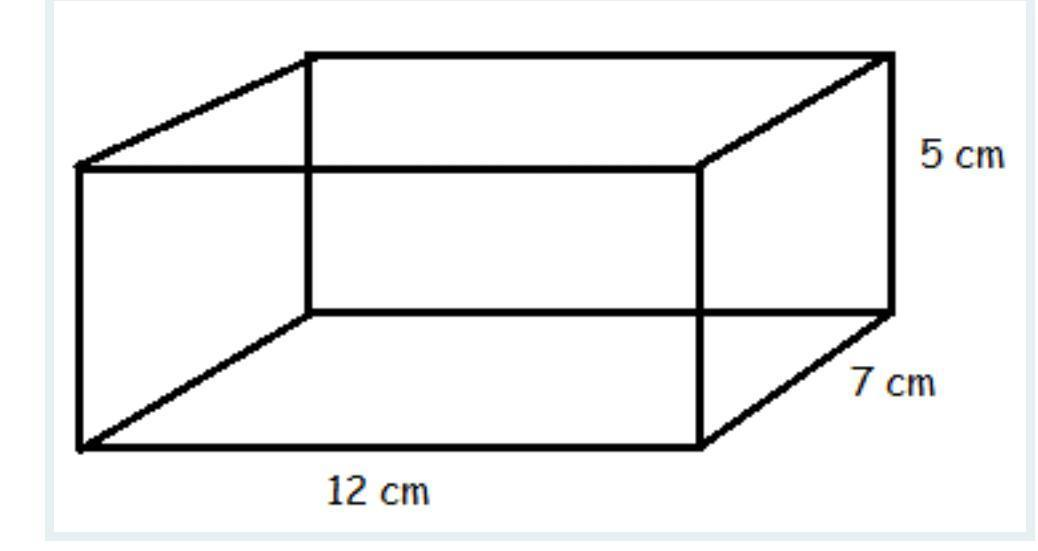
\includegraphics[width=\textwidth]{./imgSAEB_7_MAT/media/image99.jpg}
\end{figure}

\begin{escolha}
\item 24 cm³ 
\item 24 cm² 
\item 420 cm³ 
\item 420 cm²
\end{escolha}


%\section{BNCC: EF07MA30 }
% -- Resolver e elaborar problemas de cálculo de medida do
% volume de blocos retangulares, envolvendo as unidades usuais (metro
% cúbico, decímetro cúbico e centímetro cúbico).
% SAEB: Resolver problemas que envolvam volume de prismas retos ou
% cilindros retos.

% A - Incorreta, pois considerou que o volume de um bloco retangular é a
% soma das três medidas.
% B - Incorreta, pois além de somar as três medidas, a unidade está
% errada.
% C - Correta, pois, como o volume de um bloco retangular é o produto das
% medidas dos seus lados, temos que
% V = 12 \times 7 \times 5 = 420\text{cm}³.
% D - Incorreta, pois, apesar de o valor do volume ter sido calculado
% corretamente, a unidade de medida está errada.

\num{8} Ao analisar uma tabela de dupla entrada que apresenta a relação entre
o nível de escolaridade e a renda média mensal dos indivíduos, é
possível inferir a finalidade da pesquisa estatística realizada. Qual
das opções abaixo representa corretamente a finalidade dessa pesquisa?

\begin{escolha}
\item Investigar a relação entre a idade e a renda dos indivíduos.
\item Comparar a escolaridade entre diferentes faixas etárias.
\item Identificar os fatores determinantes do nível de escolaridade.
\item Avaliar a influência da escolaridade na renda dos indivíduos.
\end{escolha}


%\section{BNCC: EF07MA37 }
% -- Interpretar e analisar dados apresentados em gráfico
% de setores divulgados pela mídia e compreender quando é possível ou
% conveniente sua utilização.
% SAEB: Inferir a finalidade da realização de uma pesquisa estatística ou
% de um levantamento, dada uma tabela (simples ou de dupla entrada) ou
% gráfico, (barras simples ou agrupadas, colunas simples ou agrupadas,
% pictóricos, de linhas, de setores ou em histograma) com os dados dessa
% pesquisa.

% A - Incorreta, pois o gráfico não faz essa relação.
% B - Correta, pois o gráfica não apresenta faixas etárias.
% C - Incorreta, pois o gráfico não apresenta tais fatores.
% D - Correta, pois a tabela de dupla entrada apresenta a relação entre
% duas variáveis: o nível de escolaridade e a renda média mensal. A
% finalidade dessa pesquisa é analisar e inferir como o nível de
% escolaridade influencia a renda dos indivíduos. Ao cruzar os dados da
% tabela, é possível observar se há uma relação entre a escolaridade e a
% renda e, assim, avaliar a influência dessa variável na determinação da
% renda média mensal.

\num{9} Dia de quinta-feira é dia de jogar RPG na casa de Pedro. Considerando
que um dado de RPG tem 12 lados, qual é a chance de Pedro tirar o número
4 duas vezes seguidas?

\begin{escolha}
\item $\frac{1}{2}$
\item $\frac{2}{12}$
\item $\frac{1}{12}$
\item $\frac{1}{144}$
\end{escolha}


%\section{BNCC: EF07MA34 }
% -- Planejar e realizar experimentos aleatórios ou
% simulações que envolvem cálculo de probabilidades ou estimativas por
% meio de frequência de ocorrências.
% SAEB: Resolver problemas que envolvam a probabilidade de ocorrência de
% um resultado em eventos aleatórios equiprováveis independentes ou
% dependentes.

% A - Incorreta, pois foi feito o cálculo de probabilidade normal, sem
% considerar os eventos e considerando que o dado havia sido jogado uma
% única vez.
% B - Incorreta, pois foi feito o cálculo de uma probabilidade normal sem
% considerar os eventos.
% C - Incorreta, pois foi calculada a probabilidade de acertar a face
% número 4 uma vez.
% D - Correta, pois são eventos independentes. Desse modo:
% P\left( A \right) \times P\left( B \right) = \frac{1}{12} \times \frac{1}{12}\  = \frac{1}{144}.

\num{10} Em uma festa na escola, cada aluno levou um cupcake para comemorar.
Juliana comeu somente a metade de seu doce e cedeu o resto a Leonardo.
Como Leonardo já havia comido o dele, qual fração representa o que ele
consumiu?

\begin{escolha}
\item $\frac{1}{8}$
\item $\frac{1}{2}$
\item $1\frac{1}{2}$
\item $5\frac{1}{5}$
\end{escolha}


%\section{BNCC: EF07MA09 }
% -- Utilizar, na resolução de problemas, a associação
% entre razão e fração, como a fração 2/3 para expressar a razão de duas
% partes de uma grandeza para três partes da mesma ou três partes de outra
% grandeza.
% SAEB: Representar frações menores ou maiores que a unidade por meio de
% representações pictóricas ou associar frações a representações
% pictóricas.

% A - Incorreta, pois, o cupcake não estava dividido em oito pedaços.
% B - Incorreta, pois Leonardo consumiu mais de um cupcake.
% C - Correta, pois foi consumido 1 cupcake inteiro e metade do de
% Juliana.
% D - Incorreta, pois Leonardo não consumiu 5 cupcakes inteiros e 1 parte
% entre 4 de outro.

\num{11} A idade de Alice triplicada e somada a 19 é igual a 40. Quantos anos
ela tem?

\begin{escolha}
\item 3
\item 7
\item 20
\item 40
\end{escolha}



%\section{BNCC: EF07MA18 }
% -- Resolver e elaborar problemas que possam ser
% representados por equações polinomiais de 1º grau, redutíveis à forma ax
% + b = c, fazendo uso das propriedades da igualdade.
% SAEB: Resolver uma equação polinomial de 1º grau.

% A - Incorreta, pois, se a idade de Alice fosse 3, a idade seria igual a
% 18.
% B - Correta, pois:
% 3x + 19 = 40 \Rightarrow \ 3x = 40 - 19 - \Rightarrow 3x = 21 \Rightarrow x = 7.
% C - Incorreta, pois, se a idade de Alice fosse 20, a soma teria que ser
% 79.
% D - Incorreta, pois, se a idade de Alice fosse 40, a soma teria que ser
% 139.

\num{12} Uma bailarina está no centro de um círculo na primeira posição do
balé, ou seja, com os pés em formato de V. Se o ângulo aberto é de 30º,
quanto vale o arco correspondente?

\begin{escolha}
\item 15º
\item 17º
\item 30º
\item 60º
\end{escolha}



%\section{BNCC: EF07MA20 }
% -- Reconhecer e representar, no plano cartesiano, o
% simétrico de figuras em relação aos eixos e à origem.
% SAEB: Reconhecer circunferência/círculo como lugares geométricos, seus
% elementos (centro, raio, diâmetro, corda, arco, ângulo central, ângulo
% inscrito).

% A - Incorreta, pois o ângulo não equivale à metade de 30º.
% B - Incorreta, pois esse valor não condiz ao que foi pedido.
% C - Correta, pois, quando o ponto está no centro da circunferência, ele
% apresenta o mesmo tamanho do arco.
% D - Incorreta, pois não equivale o dobro do ângulo.

\num{13} Considere a figura A no plano cartesiano dada por A(2,3). Após a
aplicação da seguinte transformação geométrica, a figura A se transforma
na figura B:

Reflexão em relação ao eixo y, seguida de uma translação de 4 unidades
para a esquerda e 2 unidades para baixo.

Qual é a coordenada da figura B no plano cartesiano?

\begin{escolha}
\item $B(-6,1)$
\item $B(2,-5)$
\item $B(-2,1)$
\item $B(6,-1)$
\end{escolha}


%\section{BNCC: EF07MA20 }
% -- Reconhecer e representar, no plano cartesiano, o
% simétrico de figuras em relação aos eixos e à origem.
% SAEB: Identificar, no plano cartesiano, figuras obtidas por uma ou mais
% transformações geométricas (reflexão, translação, rotação).

% A - Correta, pois a reflexão em relação ao eixo y faz com que o ponto
% A(2,3) se transforme no ponto A'(-2,3). Em seguida, a translação de 4
% unidades para a esquerda e 2 unidades para baixo transforma o ponto
% A'(-2,3) no ponto B(-6,1).
% B - Incorreta, pois não leva em consideração a reflexão em relação ao
% eixo y.
% C - Incorreta, pois não leva em consideração a reflexão em relação ao
% eixo y.
% D - Incorreta, pois não leva em consideração a translação de 4 unidades
% para a esquerda e 2 unidades para baixo.

\num{14} Foi pedido a Fernanda que desenhasse um gráfico de uma equação de
primeiro grau. O gráfico de Fernanda tem de parecer com qual dos
gráficos abaixo?

\begin{escolha}
\item 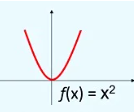
\includegraphics{./imgSAEB_7_MAT/media/image102.png}
\item 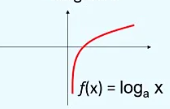
\includegraphics{./imgSAEB_7_MAT/media/image103.png}
\item 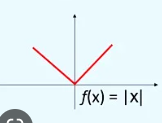
\includegraphics{./imgSAEB_7_MAT/media/image104.png}
\item 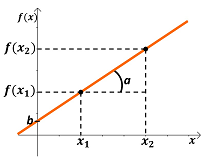
\includegraphics{./imgSAEB_7_MAT/media/image105.png}
\end{escolha}


%\section{BNCC: EF07MA18 }
% -- Resolver e elaborar problemas que possam ser
% representados por equações polinomiais de 1º grau, redutíveis à forma ax
% + b = c, fazendo uso das propriedades da igualdade.
% SAEB: Associar uma equação polinomial de 1º grau com duas variáveis a
% uma reta no plano cartesiano.

% A - Incorreta, pois é um gráfico de equação de segundo grau.
% B - Incorreta, pois é um gráfico de logarítmica
% C - Incorreta, pois é um gráfico modular
% D - Correta: pois se trata de uma reta.

\num{15} Considerando a expressão algébrica s - 15 = 2t, o valor de s
para t = 8\  é:

\begin{escolha}
\item - 5
\item 25
\item 31
\item 1
\end{escolha}


%\section{BNCC: EF07MA13 }
% -- Compreender a ideia de variável, representada por
% letra ou símbolo, para expressar relação entre duas grandezas,
% diferenciando-a da ideia de incógnita.
% SAEB: Resolver problemas que envolvam cálculo do valor numérico de
% expressões algébricas.

% A - Incorreta, pois, ao invés de multiplicar o valor de t por 2, fez a
% soma e subtraiu o 15 ao invés de somar.
% B - Incorreta, pois ao invés de multiplicar o valor de t por 2 fez a
% soma.
% C - Correta, pois, para encontrar o valor de s, basta substituir o valor
% de t dado. Assim, s - 15 = 2t\  \rightarrow \ s - 15 = 2\  \times \ 8\  \rightarrow \ s - 15 = 16\  \rightarrow \ \ s = 16 + 15 = 31.
% D - Incorreta, pois ao invés de fazer 16 + 15, fez 16-15.
\pagebreak

\mbox{}

\begin{figure}
\vspace*{-3cm}
\hspace*{-3.7cm}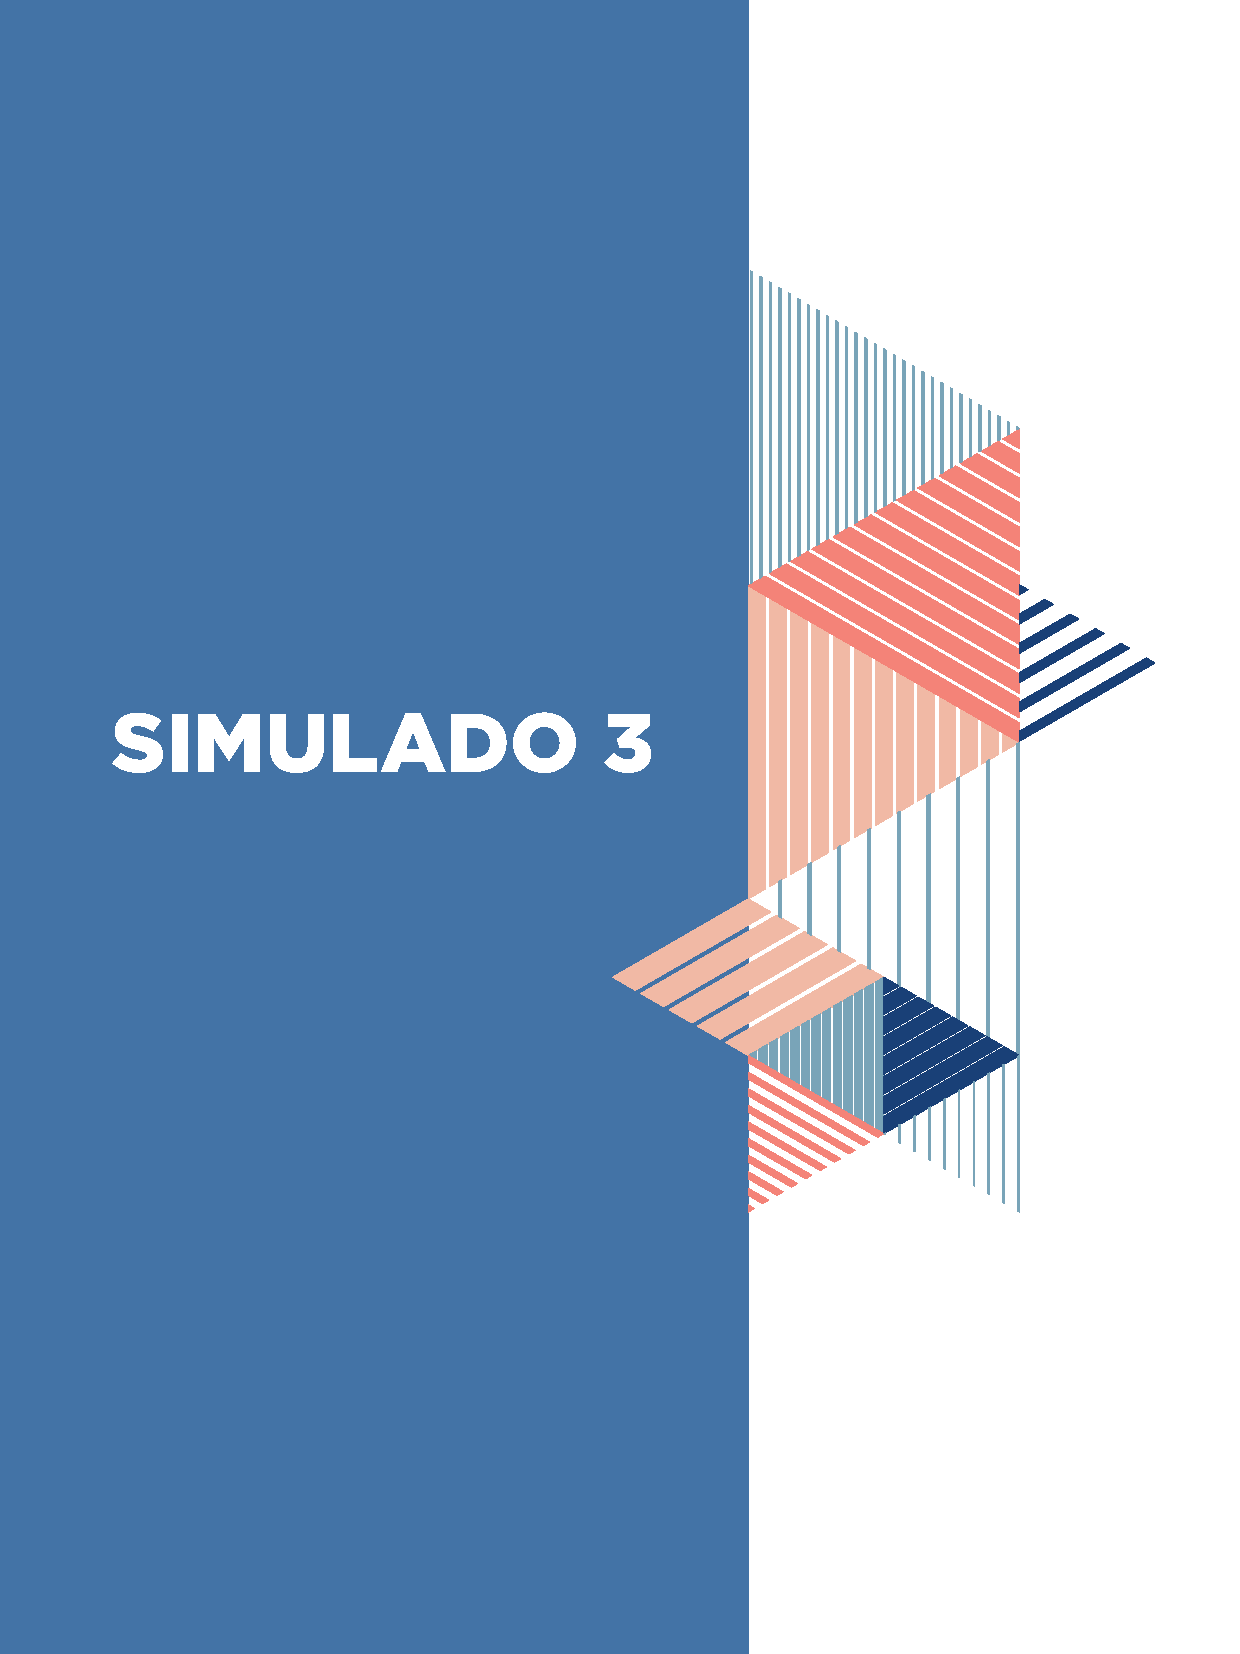
\includegraphics[scale=1]{../watermarks/3simulado9ano.pdf}
\end{figure}


\pagebreak

\section*{Simulado 3}

\num{1} Fabrício colocou em uma tabela o lucro de todos os dias da semana do
seu restaurante. Em quais dias da semana o lucro foi superior a R\$400
reais?

\begin{longtable}[]{@{}ll@{}}
\toprule
\endhead
Dias da semana & Lucro\tabularnewline
Segunda-feira & R\$100\tabularnewline
Terça-feira & R\$80\tabularnewline
Quarta-feira & R\$407\tabularnewline
Quinta-Feira & R\$100\tabularnewline
Sexta-feira & R\$140\tabularnewline
Sábado & R\$500\tabularnewline
Domingo & R\$700\tabularnewline
\bottomrule
\end{longtable}

\begin{escolha}
\item Quarta feira, Sábado e Domingo.
\item Somente domingo
\item Segunda feira, Quarta, Domingo
\item Terça feira, Sexta-feira
\end{escolha}


%\section{BNCC: EF07MA37 }
% -- Interpretar e analisar dados apresentados em gráfico
% de setores divulgados pela mídia e compreender quando é possível ou
% conveniente sua utilização.
% SAEB: Inferir a finalidade da realização de uma pesquisa estatística ou
% de um levantamento, dada uma tabela (simples ou de dupla entrada) ou
% gráfico, (barras simples ou agrupadas, colunas simples ou agrupadas,
% pictóricos, de linhas, de setores ou em histograma) com os dados dessa
% pesquisa.

% A - Correta, pois, nesses dias, o lucro foi de 407, 500 e 700,
% respectivamente.
% B - Incorreta, pois não levou em conta todo os dias em que o lucro foi
% maior.
% C - Incorreta, pois não levou em conta todo os dias em que o lucro foi
% maior.
% D - Incorreta, pois não levou em conta todo os dias em que o lucro foi
% maior.

\num{2} Luana e Gabriel estavam brincando de cara ou coroa. Qual é a chance
de Luana lançar a moeda e obter duas vezes cara?

\begin{escolha}
\item $\frac{1}{2}$
\item $\frac{2}{4}$
\item $ \frac{1}{8}$
\item $\frac{1}{4}$
\end{escolha}



%\section{BNCC: EF07MA34 }
% -- Planejar e realizar experimentos aleatórios ou
% simulações que envolvem cálculo de probabilidades ou estimativas por
% meio de frequência de ocorrências.
% SAEB: Resolver problemas que envolvam a probabilidade de ocorrência de
% um resultado em eventos aleatórios equiprováveis independentes ou
% dependentes.

% A - Incorreta, pois foi feito o cálculo da probabilidade de uma única
% moeda.
% B - Incorreta, pois não considerou cada lance como um evento
% independente.
% C - Incorreta, pois o espaço amostral não pode ser 8.
% D - Correta, pois são eventos independentes, logo
% P\left( A \right) \times P\left( B \right) = \frac{1}{2}\  \times \frac{1}{2} = \frac{1}{4}.

\num{3} 31 pessoas consumiram 8 pizzas de 8 pedaços cada e outros 2 pedaços.
Como podemos representar essa quantidade em fração?

\begin{escolha}
\item $\frac{1}{8}$
\item $\ 4\frac{1}{3}$
\item $\ 8\frac{1}{4}$
\item $\ 7\frac{1}{2}$
\end{escolha}


%\section{BNCC: EF07MA09}
%  -- Utilizar, na resolução de problemas, a associação
% entre razão e fração, como a fração 2/3 para expressar a razão de duas
% partes de uma grandeza para três partes da mesma ou três partes de outra
% grandeza.
% SAEB: Representar frações menores ou maiores que a unidade por meio de
% representações pictóricas ou associar frações a representações
% pictóricas.

% A - Incorreta, pois essa fração corresponde a comer somente 1 pedaço da
% pizza.
% B - Incorreta, pois essa fração corresponde a 4 pizzas inteiras e um
% pedaço em uma pizza de corte diferente.
% C - Correta, pois é uma fração imprópria com a parte inteira 8 e mais os
% dois pedaços.
% D - Incorreta, pois essa fração corresponde a 7 pizzas inteiras e metade
% de outra.

\num{4} Pensei em um número. Multipliquei por 3 e somei com 70, obtendo 103.
Qual é esse número?

\begin{escolha}
\item 12
\item 11
\item 20
\item 103
\end{escolha}


%\section{BNCC: EF07MA18 }
% -- Resolver e elaborar problemas que possam ser
% representados por equações polinomiais de 1º grau, redutíveis à forma ax
% + b = c, fazendo uso das propriedades da igualdade.
% SAEB: Resolver uma equação polinomial de 1º grau.

% A- Incorreta, pois, se o número fosse 12, a soma seria 106.
% B - Correta, pois 3x + 70 = 103 \rightarrow \ 3x = 103 - 70 \rightarrow \ 3x = 33 \rightarrow x = 11.
% C - Incorreta, pois, se o número fosse 20, a soma teria que ser 130.
% D - Incorreta, pois, se o número fosse 103, a soma teria que ser 379.

\num{5} Considere uma circunferência de raio 8 cm. Determine o arco
correspondente a um ângulo central de 45 graus.

\begin{escolha}
\item 2 cm
\item 6 cm
\item 8 cm
\item 16 cm
\end{escolha}



%\section{BNCC: EF07MA21 }
% -- Reconhecer e construir figuras obtidas por simetrias
% de translação, rotação e reflexão, usando instrumentos de desenho ou
% softwares de geometria dinâmica e vincular esse estudo a representações
% planas de obras de arte, elementos arquitetônicos, entre outros.
% SAEB: Reconhecer circunferência/círculo como lugares geométricos, seus
% elementos (centro, raio, diâmetro, corda, arco, ângulo central, ângulo
% inscrito).

% A - Incorreta, pois essa resposta não corresponde ao cálculo correto do
% arco.
% B - Correta, pois o arco correspondente ao ângulo central de 45 graus
% possui um comprimento de aproximadamente 6.28 cm.
% C - Incorreta, pois essa resposta corresponde ao perímetro da
% circunferência, não ao comprimento do arco de um ângulo central
% específico.
% D - Incorreta, pois essa resposta corresponde ao dobro do perímetro da
% circunferência, não ao comprimento do arco de um ângulo central
% específico.

\num{6} Dois corredores saem da linha de partida ao mesmo tempo. Sabendo que
um deles percorre toda a pista em 15 minutos e o outro, em 25 minutos,
dentro de quanto tempo eles se encontram novamente na linha de partida?

\begin{escolha}
\item 5 minutos
\item 40 minutos.
\item 1 hora e 5 minutos
\item 1 hora e 15 minutos
\end{escolha}


%\section{BNCC: EF07MA04 }
% -- Resolver e elaborar problemas que envolvam operações
% com números inteiros.
% SAEB: Resolver problemas que envolvam as ideias de múltiplo, divisor,
% máximo divisor comum ou mínimo múltiplo comum.

% A - Incorreta, pois considerou que o tempo de encontro seria pelo M.D.C
% ao invés do M.M.C. . B - Incorreta, pois apenas foi feita a soma do
% tempo de cada corredor. C - Incorreta, pois foi associado um número
% errado de minutos. D - Correta, pois devemos usar a ideia de mínimo
% múltiplo comum. Assim, calculando o M.M.C dos tempos, temos: 15, 25, 3; 5, 25, 5; 1, 5, 5; 1, 1, (3x5x5 = 75). Logo, os atletas se encontram depois de 75 minutos, ou seja, 1 hora e 15
% minutos.

\num{7} A porcentagem possui diversas representações: a percentual, a
fracionária e a decimal. Considerando a porcentagem, 25,3\% as suas
representações são:

\begin{escolha}
\item 2,53 e $\frac{253}{100} $
\item 0,253 e $\frac{253}{1000} $
\item 0,253 e $\frac{253}{100} $
\item 2,53 e $\frac{253}{1000}$
\end{escolha}


%\section{BNCC: EF07MA02 }
% --: Resolver e elaborar problemas que envolvam
% porcentagens, como os que lidam com acréscimos e decréscimos simples,
% utilizando estratégias pessoais, cálculo mental e calculadora, no
% contexto de educação financeira, entre outros.
% SAEB: - Resolver problemas que envolvam porcentagens, incluindo os que
% lidam com acréscimos e decréscimos simples, aplicação de percentuais
% sucessivos e determinação de taxas percentuais.

% A - Incorreta, pois considerou que o numerador da fração centesimal é a
% forma percentual sem a vírgula.
% B - Correta, pois
% 25,3\% = \frac{25,3}{100} = \frac{253}{1000} = 0,253.
% C - Incorreta, pois esqueceu de adicionar um 0 no denominador da
% representação fracionária ao andar com a vírgula.
% D - Incorreta, pois se esqueceu de levar em conta as 3 casas decimais no
% denominador.

\num{8} A corrida de um táxi na cidade de São Paulo custa
R\$ 1,50 por km rodado mais a bandeira de R\$ 6,50. Uma pessoa que pagou
R\$ 18,50 por uma corrida percorreu um total de:

\begin{escolha}
\item 18 km
\item 16,6 km
\item 12,3km 
\item 8 km
\end{escolha}


%\section{BNCC: EF07MA13 }
% -- Compreender a ideia de variável, representada por
% letra ou símbolo, para expressar relação entre duas grandezas,
% diferenciando-a da ideia de incógnita.
% SAEB: Resolver problemas que envolvam cálculo do valor numérico de
% expressões algébricas.

% A - Incorreta, pois ao invés de fazer \frac{12}{1,5}\ calculou 12 x
% 1,5. B - Incorreta, pois ao invés de fazer 18,5 - 6,5 fez uma soma. C -
% Incorreta, pois considerou apenas o preço pago por km sem o valor da
% bandeira. D - Correta, pois, como a corrida tem um preço por km mais um
% fixo, podemos escrever de maneira geral que a corrida custa
% c = 1,5q + 6,5. Assim, 18,5 = 1,5q + 6,5 \rightarrow 1,5q = 12 \rightarrow \ q = \frac{12}{1,5} \rightarrow q = 8\text{km}.

\num{9} Um atendente de um banco gasta 1 horas e 40 minutos para atender 12
clientes. No quinto dia útil o atendimento acaba sendo maior, então para
atender 18 clientes, o atendente vai gastar:

\begin{escolha}
\item 2 horas e 30 minutos
\item 1 hora e 30 minutos
\item 1 hora e 7 minutos
\item 1 hora e 50 minutos
\end{escolha}


%\section{BNCC: EF07MA17 }
% -- Resolver e elaborar problemas que envolvam variação de
% proporcionalidade direta e de proporcionalidade inversa entre duas
% grandezas, utilizando sentença algébrica para expressar a relação entre
% elas.
% SAEB: Resolver problemas que envolvam variação de proporcionalidade
% direta~ou inversa entre duas ou mais grandezas.

% A - Correta, pois, quanto mais pessoas para atender, mais tempo será
% gasto, logo são G.D.P. Para fazer o cálculo, precisamos do tempo em uma
% unidade apenas, ou seja, 1 hora e 40 minutos será 100 minutos. Assim, \frac{100}{12} = \frac{x}{18} \rightarrow 12x = 1800 \rightarrow x = \frac{1800}{12} = 150\ \text{minutos} = 2\ h\text{oras}\ e\ 30\ \text{minutos}. B - Incorreta, pois, ao converter 150 minutos para horas, considerou 1
% hora ao invés de 2. C - Incorreta, pois considerou as grandezas como sendo inversamente
% proporcionais, fazendo 100\ .\ 12\  = \ 18x. D - Incorreta, pois considerou que 1 hora tem 100 minutos.

\num{10} Considere um triângulo ABC, onde AB = 8 cm, AC = 6 cm e BC = 10 cm.
Qual é a medida da altura relativa ao lado AB?

\begin{escolha}
\item 2 cm
\item 3 cm
\item 4 cm
\item 5 cm
\end{escolha}



%\section{BNCC: EF07MA23 }
% -- Verificar relações entre os ângulos formados por retas
% paralelas cortadas por uma transversal, com e sem uso de softwares de
% geometria dinâmica.
% SAEB: Resolver problemas que envolvam relações entre ângulos formados
% por retas paralelas cortadas por uma transversal, ângulos internos ou
% externos de polígonos ou cevianas (altura, bissetriz, mediana,
% mediatriz) de polígonos.

% A - Incorreta, pois 2 cm é a medida da altura relativa ao lado BC.
% B - Incorreta, pois 3 cm é a medida da altura relativa ao lado AC.
% C - Correta, pois a altura relativa ao lado AB divide o triângulo ABC em
% dois triângulos retângulos, onde a altura é a hipotenusa e os catetos
% são os segmentos AH e BH. Podemos utilizar o teorema de Pitágoras para
% calcular a medida da altura e chegar ao resultado.
% D - Incorreta, pois 5 cm é a medida da mediana relativa ao lado AB.

\num{11} Qual das seguintes afirmações melhor descreve a diferença entre
mapa, planta e croqui?

\begin{escolha}
\item Um mapa é uma representação de uma região ou área, enquanto uma planta é um desenho esquemático de uma construção, e um croqui é uma vista aérea de uma cidade ou paisagem.
\item Um mapa é uma vista aérea de uma cidade ou paisagem, enquanto uma planta é uma representação de uma região ou área, e um croqui é um desenho esquemático de uma construção.
\item Um mapa é um desenho esquemático de uma construção, enquanto uma planta é uma representação de uma região ou área, e um croqui é uma vista aérea de uma cidade ou paisagem.
\item Um mapa, uma planta e um croqui são todos sinônimos e podem ser usados de forma intercambiável.
\end{escolha}


% SAEB: Descrever ou esboçar deslocamento de pessoas e/ou de objetos em
% representações bidimensionais (mapas, croquis etc.), plantas de
% ambientes ou vistas, de acordo com condições dadas.

% A - Correta, pois essa definição está correta.
% B - Incorreta, pois as primeiras definições estão incorretas.
% C - Incorreta, pois a definição de planta está incorreta.
% D - Incorreta, pois há diferenças entre esses conceitos.

\num{12} Qual é a área de um triângulo retângulo com base de 10 cm e altura
de 6 cm?

\begin{escolha}
\item 30 cm²
\item 36 cm²
\item 45 cm²
\item 60 cm²
\end{escolha}


%\section{BNCC: EF07MA31 }
% -- Estabelecer expressões de cálculo de área de
% triângulos e de quadriláteros.
% SAEB: Resolver problemas que envolvam área de figuras planas.

% A - Incorreta, pois essa resposta corresponde ao cálculo incorreto da
% área.
% B - Correta, pois, substituindo os valores fornecidos na fórmula, temos:
% Área do triângulo = \frac {(10 \times 6)}{2} = \frac {60}{2} =
% 30 \;cm^2. Portanto, a área do triângulo retângulo é de 30 cm².
% A = \frac{\left( b + B \right)h}{2} = \frac{(6 + 18) \times 10}{2} = 24 \times 5 = 120m².
% C - Incorreta, pois essa resposta não corresponde ao cálculo correto da
% área do triângulo com os valores fornecidos.
% D - Incorreta, pois essa resposta corresponde à multiplicação da base
% pela altura, sem dividir por 2, o que resulta em uma área incorreta.

\num{13} Em um plano cartesiano, foi desenhada uma letra L no primeiro
quadrante. Se eu desenhar a mesma letra com as mesmas dimensões, mas sem
utilizar da simetria dos pares ordenados, com duas unidades para cima,
qual transformação geométrica ocorrerá?

\begin{escolha}
\item Translação
\item Rotação
\item Reflexão
\item Imersão
\end{escolha}


%\section{BNCC: EF07MA20 }
% -- Reconhecer e representar, no plano cartesiano, o
% simétrico de figuras em relação aos eixos e à origem.
% SAEB: Identificar, no plano cartesiano, figuras obtidas por uma ou~ mais
% transformações geométricas (reflexão, translação, rotação).

% A - Correta, pois como não saiu do eixo e só subiu duas unidades da
% simetria, ocorreu a translação.
% B - Incorreta, pois, para ocorrer a rotação, teríamos uma inclinação.
% C - Incorreta, pois a transformação geométrica reflexão apenas repetiria
% a figura.
% D - Incorreta, pois a imersão não é uma transformação geométrica.

\num{14} Em uma competição de natação, Renato, Yan, Cristian e Rafael
completaram as provas, respectivamente, nos seguintes tempos: 7,573
7,563 7,482 7,568. Quem foi o terceiro colocado entre eles?

\begin{escolha}
\item Yan
\item Renato
\item Cristian
\item Rafael
\end{escolha}



%\section{BNCC: EF07MA10 }
% -- Comparar e ordenar números racionais em diferentes
% contextos e associá-los a pontos da reta numérica.
% SAEB: Comparar ou ordenar números reais, com ou sem suporte da reta
% numérica, ou aproximar número reais para múltiplos de potência de 10
% mais próxima.

% A - Incorreta, pois Yan é o segundo colocado.
% B- Incorreta, pois Renato é o último colocado.
% C - Incorreta, pois Cristian ficou em primeiro lugar.
% D - Correta, pois Rafael ficou na terceira posição.

\num{15} Considerando a expressão algébrica $x - y + 20 = 0$, o valor de x
para y = - 2 é:

\begin{escolha}
\item 22
\item - 22
\item - 18
\item 18
\end{escolha}

%\section{BNCC: EF07MA13 }
% -- Compreender a ideia de variável, representada por
% letra ou símbolo, para expressar relação entre duas grandezas,
% diferenciando-a da ideia de incógnita.
% SAEB: Resolver problemas que envolvam cálculo do valor numérico de
% expressões algébricas.

% A - Incorreta, pois não trocou a operação do 22 ao mudar de lado na
% igualdade.
% B - Correta, pois, para encontrar o valor de x, basta substituir o valor
% de y. Assim, x - y + 20 = 0 \rightarrow x - ( - 2) + 20 = 0 \rightarrow \ x + 22 = 0 \rightarrow \ x = - 22.
% C - Incorreta, pois, ao substituir o y, a mudança de sinal não foi
% feita.
% D - Incorreta, pois, além de não fazer a mudança do sinal com o y, a
% operação do 18 não foi feita.


\pagebreak

\mbox{}

\begin{figure}
\vspace*{-3cm}
\hspace*{-3.7cm}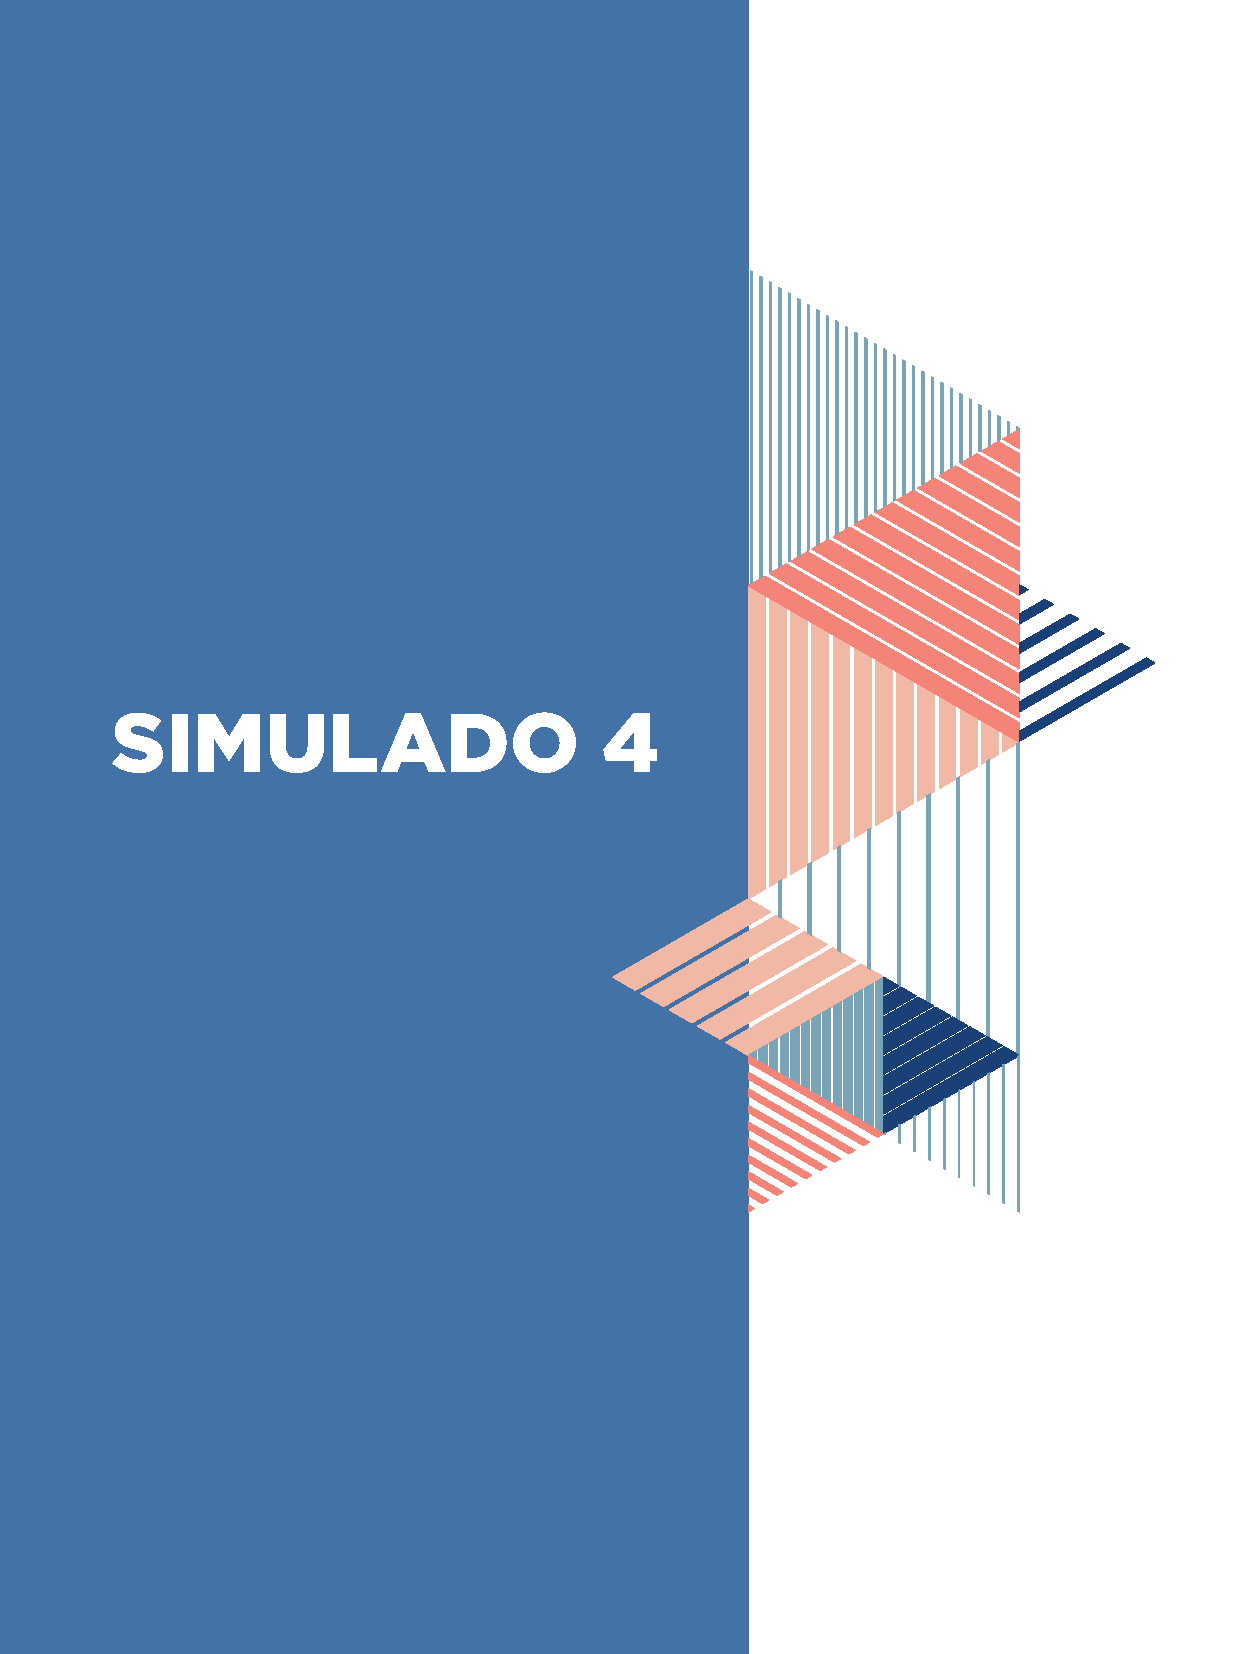
\includegraphics[scale=1]{../watermarks/4simulado9ano.pdf}
\end{figure}


\pagebreak

\section*{Simulado 4}

\num{1} Em uma corrida, o primeiro lugar ganhou com diferença de 0,035 de
tempo para o segundo lugar. A diferença de tempo por extenso é:

\begin{escolha}
\item~35 segundos
\item 35 milésimos de segundos
\item 35 centésimos de segundos
\item 35 minutos
\end{escolha}

%\section{BNCC: EF07MA10 }
% -- Comparar e ordenar números racionais em diferentes
% contextos e associá-los a pontos da reta numérica.
% SAEB: Escrever números racionais (representação fracionária ou decimal
% finita) em sua representação por algarismos ou em língua materna ou
% associar o registro numérico ao registro em língua materna.

% A - Incorreta, pois 35 segundos não é representado por números decimais.
% B - Correta, pois, quando há três casas decimais, temos milésimos de
% segundos.
% C - Incorreta, pois 35 centésimos de segundos apareceria com duas casas
% decimais após a vírgula.
% D - Incorreta, pois 3 minutos é uma quantidade representada por um
% número inteiro.

\num{2} A data para a eleição do novo diretor da escola foi marcada para o
final do mês de novembro. A escola possui 9 turmas, sendo que somente
uma turma de 9º ano ainda não pode votar. Duas alunas tiveram a ideia de
pesquisar a intenção de voto de algumas pessoas, angariando a opinião de
3 turmas completas. Marque a opção que indica, respectivamente, a
população e a amostra dessa pesquisa.

\begin{escolha}
\item 9 turmas, 3 turmas
\item 3 turmas, 9 turmas
\item 8 turmas, 3 turmas
\item 3 turmas, 8 turmas
\end{escolha}


%\section{BNCC: EF07MA35 }
% -- Compreender, em contextos significativos, o
% significado de média estatística como indicador da tendência de uma
% pesquisa, calcular seu valor e relacioná-lo, intuitivamente, com a
% amplitude do conjunto de dados.
% SAEB: Identificar os indivíduos (universo ou população-alvo da
% pesquisa), as variáveis e os tipos de variáveis (quantitativas ou
% categóricas) em um conjunto de dados.

% A - Incorreta, pois, apesar de a escola ter 9 turmas, uma delas é
% excluída da votação.
% B - Incorreta, pois o valor de amostra e população estão invertidos.
% C - Correta, pois temos 8 turmas como população e 3 turmas de amostra.
% D - Incorreta, pois o valor da amostra e população estão invertidos.

\num{3} Ana Clara encheu $\frac{4}{8}$ do galão de água da casa dela. Um
valor equivalente seria

\begin{escolha}
\item Metade
\item Inteiro
\item $\frac{1}{4}$
\item $\frac{1}{3}$
\end{escolha}


%\section{BNCC: EF07MA08}
%  -- Comparar e ordenar frações associadas às ideias de
% partes de inteiros, resultado da divisão, razão e operador.
% SAEB:~Identificar frações equivalentes.

% A - Correta, pois \frac{4}{8} é equivalente a \frac{1}{2}.
% B - Incorreta, pois a fração não corresponde ao galão inteiro, uma vez
% que encheu 4 partes de 8 divididas.
% C - Incorreta, pois a fração irredutível encontrada está errada.
% D - Incorreta, pois essa fração não representa a parte cheia do galão.

\num{4} Yuri pensou em um número que, somado a 1.200, é igual a quatro vezes
si mesmo. O número que Yuri pensou é:

\begin{escolha}
\item 355
\item 400
\item 200
\item 420
\end{escolha}

%\section{BNCC: EF07MA18}
%  -- Resolver e elaborar problemas que possam ser
% representados por equações polinomiais de 1º grau, redutíveis à forma ax
% + b = c, fazendo uso das propriedades da igualdade.
% SAEB: Resolver uma equação polinomial de 1º grau.

% A - Incorreta, pois, se o número fosse 355, o resultado final seria
% diferente.
% B - Correta, pois
% x + 1200 = 4x \rightarrow \ 4x - x = 1200 \rightarrow 3x = 1200 \rightarrow x = 400.
% C - Incorreta, pois, se o número fosse 200, o resultado final seria
% diferente.
% D - Incorreta, pois, se o número fosse 420, o resultado final seria
% diferente.

\num{5} Qual é o arco de uma circunferência de raio 10 cm, considerando um
ângulo central de 60°?

\begin{escolha}
\item 10\pi cm
\item 6\pi cm
\item 3\pi cm
\item 2\pi cm
\end{escolha}


%\section{BNCC: EF07MA19 }
% -- Realizar transformações de polígonos representados no
% plano cartesiano, decorrentes da multiplicação das coordenadas de seus
% vértices por um número inteiro.
% SAEB: Reconhecer circunferência/círculo como lugares geométricos, seus
% elementos (centro, raio, diâmetro, corda, arco, ângulo central, ângulo
% inscrito).

% A - Incorreta, pois o valor do ângulo central não foi considerado
% corretamente.
% B - Incorreta, pois o valor do ângulo central não foi considerado
% corretamente.
% C - Correta, pois Arco = \frac {Ângulo}{360º} \times 2π \times raio.
% No caso do problema, substituindo os valores na fórmula, temos 3π cm.
% D - Incorreta, pois o valor do ângulo central não foi considerado
% corretamente.

\num{6} A transformação geométrica que ocorre com objetos bidimensionais
posicionados diante de um espelho perpendicular é:

\begin{escolha}
\item Rotação
\item Reflexão
\item Translação
\item Inchaço
\end{escolha}

%\section{BNCC: EF07MA20}
%  -- Reconhecer e representar, no plano cartesiano, o
% simétrico de figuras em relação aos eixos e à origem.
% SAEB: Identificar, no plano cartesiano, figuras obtidas por uma ou~ mais
% transformações geométricas (reflexão, translação, rotação).

% A - Incorreta, pois a rotação acontece quando o objeto inclina-se.
% B - Correta, pois o ato de posicionar um espelho reflete a imagem.
% C - Incorreta, pois a translação ocorre quando o objeto segue pelas
% direções norte, sul, leste e oeste.
% D - Incorreta, pois no inchaço há deformação na imagem.

\num{7} O professor de Matemática resolveu fazer uma brincadeira e contar as
notas dos alunos em forma de fração, Lúcio tirou $\frac{19}{3}$. Onde
está localizado este número na reta numérica?

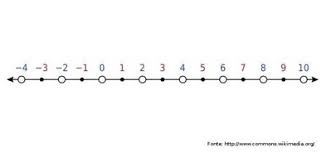
\includegraphics{./imgSAEB_7_MAT/media/image109.png}

\begin{escolha}
\item Entre o 5 e o 6
\item Entre o 9 e o 10
\item Próximo ao 1
\item Entre o 6 e o 7
\end{escolha}


%\section{BNCC: EF07MA01 }
% -- Resolver e elaborar problemas com números naturais,
% envolvendo as noções de divisor e de múltiplo, podendo incluir máximo
% divisor comum ou mínimo múltiplo comum, por meio de estratégias
% diversas, sem a aplicação de algoritmos.
% SAEB: Comparar ou ordenar números reais, com ou sem suporte da reta
% numérica, ou aproximar número reais para múltiplos de potência de 10
% mais próxima.

% A - Incorreta, pois a divisão de 19 por 3 é maior que 6.
% B - Incorreta, pois a divisão de 19 por 3 é menor que 7.
% C - Incorreta, pois a divisão de 19 por 3 é maior que 1.
% D - Correta, pois, analisando a fração como divisão, temos que o 3 está
% dentro do 9 aproximadamente 6 vezes, logo, a fração é maior do que 6 e
% menor do que 7.

\num{8} Marcos está montando uma lembrança para seus alunos e resolveu fazer
saquinhos com doces. Ele comprou 75 balas, 60 pirulitos e 45 chocolates,
e quer dividi-los com a maior quantidade possível de cada doce por
lembrancinha. Assim, em cada saquinho, o número de lembranças será

\begin{escolha}
\item 5
\item 8
\item 15
\item 20
\end{escolha}


%\section{BNCC: EF07MA04 }
% -- Resolver e elaborar problemas que envolvam operações
% com números inteiros.
% SAEB: Resolver problemas que envolvam as ideias de múltiplo, divisor,
% máximo divisor comum ou mínimo múltiplo comum.

% A - Incorreta, pois esqueceu de considerar que o 3 também dividiu os
% valores simultaneamente.
% B - Incorreta, pois, ao invés de multiplicar o 3 e o 5, fez a soma
% deles.
% C - Correta, pois, para dividir as lembranças na maior quantidade
% possível, usamos o cálculo do M.D.C; assim, fatorando a quantidade de
% cada doce, temos 75, 60, 45, 2; 75, 30, 45, 2; 75, 15, 45, 3; 25, 5, 15, 3; 25, 5, 5, 5; 5, 1, 1, 5; 1, 1, 1. Logo, em cada saquinho terá 15 doces.
% D - Incorreta, pois, ao fatorar, considerou que usaria todos os fatores
% como se fosse M.M.C.

\num{9} Larissa decidiu comprar um videogame de presente para seu sobrinho.
Fazendo uma pesquisa na internet, encontrou um valor de R\$3.500,00 com
desconto de 5\% à vista. Ela já havia procurado na cidade e encontrado o
mesmo aparelho por R\$3.800,00 com desconto de 10\% à vista. Sabendo que
a loja virtual cobra um frete de R\$35,00 e que Larissa vai comprar à
vista, a melhor opção dela é:

\begin{escolha}
\item Na loja virtual, pagando R\$3.360,00
\item Na loja virtual, pagando R\$3.325,00
\item Na loja física, pagando R\$3.360,00 
\item Na loja física, pagando R\$3.420,00
\end{escolha}


%\section{BNCC: EF07MA02 }
%-- Resolver e elaborar problemas que envolvam
% porcentagens, como os que lidam com acréscimos e decréscimos simples,
% utilizando estratégias pessoais, cálculo mental e calculadora, no
% contexto de educação financeira, entre outros.
% SAEB: - Resolver problemas que envolvam porcentagens, incluindo os que
% lidam com acréscimos e decréscimos simples, aplicação de percentuais
% sucessivos e determinação de taxas percentuais.

% A - Correta, pois \text{Na}\ \text{loja}\ \text{virtual} \rightarrow 3500 \times 0,95 = 3.325 + 35 = 3360. \text{Na}\ \text{loja}\ fí\text{sica} \rightarrow 3800 \times 0,9 = 3420. Portanto, a melhor opção de Larissa é a loja virtual.
% B - Incorreta, pois não considerou o valor do frete da loja virtual.
% C - Incorreta, pois confundiu as informações da loja física com a
% virtual.
% D - Incorreta, pois, ao realizar as operações, o resultado obtido é
% outro.

\num{10} Analisando as sequências abaixo, podemos classificá-las como
recursivas ou não recursivas na seguinte ordem:

\begin{enumerate}
\item $(1,\ 4,\ 7,\ 10,\ 13,\ \ldots)$
\item $( - 3,\  - 5\ , - \ 7,\  - 9,\  - 11, \ldots)$
\item $(2,\ 3,\ 5,\ 7,\ 11, \ldots)$
\end{enumerate}


\begin{escolha}
\item Recursiva, não recursiva, recursiva
\item Recursiva, recursiva, recursiva
\item Recursiva, não recursiva, não recursiva
\item Recursiva, recursiva, não recursiva
\end{escolha}

%\section{BNCC: EF07MA14}
%  -- Classificar sequências em recursivas e não recursivas,
% reconhecendo que o conceito de recursão está presente não apenas na
% matemática, mas também nas artes e na literatura.
% SAEB: Identificar uma representação algébrica para o padrão ou a
% regularidade de uma sequência de números racionais ou representar
% algebricamente o padrão ou a regularidade de uma sequência de números
% racionais.

% A - Incorreta, pois considerou que a sequência 2 não apresenta uma
% relação entre os termos e que os números primos possuem algum padrão.
% B - Incorreta, pois considerou que a sequência dos números primos pode
% ser encontrada por alguma relação entre os termos.
% C - Incorreta, pois não enxergou que a sequência 2 apresenta uma relação
% entre os termos por meio do antecessor subtraído de 2.
% D - Correta, pois podemos observar que a sequência I é determinada pelo
% termo anterior mais 3, a sequência II pelo termo anterior menos 2, e a
% III é a sequência dos números primos. Como a sequência recursiva é
% aquela em que um termo depende do anterior, temos recursiva, recursiva e
% não recursiva.

\num{11} Sabendo que $x + y + z = 38$, o valor de x, y, z na proporção
abaixo é, respectivamente:

$\frac{x}{42} = \frac{y}{16} = \frac{z}{18}$

\begin{escolha}
\item 84, 32, 36
\item 21, 8, 9
\item 84, 36, 32
\item 21, 9, 8
\end{escolha}

%\section{BNCC: EF07MA17 }
% -- Resolver e elaborar problemas que envolvam variação de
% proporcionalidade direta e de proporcionalidade inversa entre duas
% grandezas, utilizando sentença algébrica para expressar a relação entre
% elas.
% SAEB: Resolver problemas que envolvam variação de proporcionalidade
% direta~ou inversa entre duas ou mais grandezas.

% A - Incorreta, pois, ao determinar o valores de x, y, z, foi feita uma
% multiplicação por 2 ao invés de uma divisão.
% B - Correta, pois \frac{x}{42} = \frac{y}{16} = \frac{z}{18} = \frac{x + y + z}{42 + 16 + 18} = \frac{38}{76} = \frac{1}{2}. \frac{x}{42} = \frac{1}{2} \rightarrow \ \ x = 21. \frac{y}{16} = \frac{1}{2} \rightarrow \ \ x = 8\ \ \ \ \ \ \ \ \ \ \ \ \frac{z}{18} = \frac{1}{2} \rightarrow \ \ x = 9.
% C - Incorreta, pois, além de calcular o valor das incógnitas usando a
% multiplicação, os valores que seriam y e z foram invertidos.
% D - Incorreta, pois, apesar de fazer os cálculos corretos, a ordem dos
% valores de y e z foi invertida.

\num{12} Em um triângulo retângulo, a hipotenusa mede 10 cm e um dos catetos
mede 6 cm. Qual é a medida do ângulo agudo oposto a esse cateto?

\begin{escolha}
\item 30°
\item 45°
\item 60°
\item 90°
\end{escolha}


%\section{BNCC: EF07MA23 }
% -- Verificar relações entre os ângulos formados por retas
% paralelas cortadas por uma transversal, com e sem uso de softwares de
% geometria dinâmica.
% SAEB: Resolver problemas que envolvam relações entre ângulos formados
% por retas paralelas cortadas por uma transversal, ângulos internos ou
% externos de polígonos ou cevianas (altura, bissetriz, mediana,
% mediatriz) de polígonos.

% A - Incorreta, pois não corresponde à medida correta do ângulo agudo.
% B - Incorreta, pois não corresponde à medida correta do ângulo agudo.
% C - Correta, pois, no triângulo retângulo, o ângulo agudo oposto ao
% cateto é sempre o complementar do ângulo formado entre a hipotenusa e o
% cateto. Esse ângulo pode ser encontrado usando a função trigonométrica
% seno.
% D - Incorreta, pois corresponde ao ângulo reto, não ao ângulo agudo
% oposto ao cateto.

\num{13} Qual é o perímetro de um retângulo com comprimento de 10 cm e
largura de 5 cm?

\begin{escolha}
\item 10 cm
\item 15 cm
\item 20 cm
\item 30 cm
\end{escolha}

%SAEB: Resolver problemas que envolvam perímetro de figuras planas.

% A - Incorreta, pois corresponde à soma apenas dos comprimentos das duas
% arestas menores.
% B - Incorreta, pois corresponde à soma apenas dos comprimentos das duas
% arestas maiores.
% C - Correta, pois o perímetro de um retângulo é dado pela soma dos
% comprimentos de todos os lados, ou seja, a soma dos comprimentos das
% quatro arestas.
% No caso do retângulo descrito no problema, temos duas arestas de
% comprimento 10 cm e duas arestas de comprimento 5 cm. Portanto, o
% perímetro é dado por: P = 10 cm + 10 cm + 5 cm + 5 cm P = 20 cm + 10 cm P = 30 cm. 
% D - Incorreta, pois corresponde à soma de todos os lados do retângulo,
% incluindo os comprimentos das arestas duas vezes.

\num{14} Qual é a área de um triângulo retângulo com base de 8 cm e altura de
6 cm?

\begin{escolha}
\item 12 cm²
\item 24 cm²
\item 30 cm²
\item 48 cm²
\end{escolha}

%\section{BNCC: EF07MA32}
%  -- Resolver e elaborar problemas de cálculo de medida de
% área de figuras planas que podem ser decompostas por quadrados,
% retângulos e/ou triângulos, utilizando a equivalência entre áreas.
%SAEB: Resolver problemas que envolvam área de figuras planas.

% A - Incorreta, pois corresponde à metade da área correta do triângulo.
% B - Correta, pois a fórmula para calcular a área de um triângulo é dada
% pela metade do produto da base pela altura: A =
% \frac {(base \times altura)}{2}. Substituindo os valores do problema, temos: A = 24 cm².
% C - Incorreta, pois não corresponde à área correta do triângulo.
% D - Incorreta, pois corresponde à área do retângulo formado pela base e
% altura do triângulo, não à área do próprio triângulo.

\num{15} Considerando a expressão algébrica $2a + 8 - 3b = 5$, o valor de $b$
para $a = - 3$ é:

\begin{escolha}
\item $- 1$
\item $1$
\item $3$
\item $- \frac{7}{3}$
\end{escolha}

%\section{BNCC: EF07MA13 }
% -- Compreender a ideia de variável, representada por
% letra ou símbolo, para expressar relação entre duas grandezas,
% diferenciando-a da ideia de incógnita.
% SAEB: Resolver problemas que envolvam cálculo do valor numérico de
% expressões algébricas.

% A - Correta, pois, para encontrar o valor de b, basta substituir o valor
% de a. Assim, 2a + 8 - 3b = 5\  \rightarrow \ 2\  \times \ \left( - 3 \right) + 8 - 3b = 5 \rightarrow \  - 6 + 8 - 3b = 5 - 3b = 3\  \rightarrow \ b = \  - 1.
% B - Incorreta, pois, ao dividir 3 por -3, a regra de sinal não foi
% respeitada.
% C - Incorreta, pois ao fazer 2\  \times \ \left( - 3 \right), foi
% encontrado 6 ao invés de -6.
% D - Incorreta, pois, ao passar o 2 de lado, a regra do sinal foi
% ignorada.

